\documentclass{llncs}
\usepackage[title]{appendix}
\usepackage[pagebackref]{hyperref}
\usepackage{subcaption}
\usepackage{graphicx}
\usepackage{comment}
\usepackage{amsmath,amssymb} % define this before the line numbering.
\usepackage{color}

\newcommand{\reffig}[1]{\hyperref[#1]{Figure \ref*{#1}}}
\newcommand{\refsec}[1]{\hyperref[#1]{Section \ref*{#1}}}
\newcommand{\reftab}[1]{\hyperref[#1]{Table \ref*{#1}}}
\newcommand{\refapp}[1]{\hyperref[#1]{Appendix \ref*{#1}}}
\DeclareMathOperator*{\argminA}{arg\,min} % Jan Hlavacek

% INITIAL SUBMISSION - The following two lines are NOT commented
% CAMERA READY - Comment OUT the following two lines
% \usepackage{ruler}
% \usepackage[width=122mm,left=12mm,paperwidth=146mm,height=193mm,top=12mm,paperheight=217mm]{geometry}

\begin{document}
% \renewcommand\thelinenumber{\color[rgb]{0.2,0.5,0.8}\normalfont\sffamily\scriptsize\arabic{linenumber}\color[rgb]{0,0,0}}
% \renewcommand\makeLineNumber {\hss\thelinenumber\ \hspace{6mm} \rlap{\hskip\textwidth\ \hspace{6.5mm}\thelinenumber}}
% \linenumbers
\pagestyle{headings}
\mainmatter
\def\ECCVSubNumber{100}  % Insert your submission number here

\title{Towards Bringing Together Numerical Methods for Partial Differential Equation and Deep Neural Networks} % Replace with your title

% INITIAL SUBMISSION
\begin{comment}
\titlerunning{Towards Bringing Together Numerical Methods for Partial Differential Equation and Deep Neural Networks}
\authorrunning{Stanislav Arnaudov, Markus Hoffmann}
\author{Stanislav Arnaudov, Markus Hoffmann}
\institute{Karlsruhe Institute of Technology,\\Kaiserstrasse 12,76131 Karlsruhe, Germany\\ \url{http://www.kit.edu/english/}}
\end{comment}
%******************

% CAMERA READY SUBMISSION
% \begin{comment}
\titlerunning{Abbreviated paper title}
% If the paper title is too long for the running head, you can set
% an abbreviated paper title here
%
\author{Stanislav Arnaudoc, Markus Hoffmann }
%
\authorrunning{F. Author et al.}
% First names are abbreviated in the running head.
% If there are more than two authors, 'et al.' is used.
%
\institute{Karlsruhe Institute of Technology,\\Kaiserstrasse 12,76131 Karlsruhe, Germany\\ \url{http://www.kit.edu/english/}}
% \end{comment}
%******************
\maketitle

\begin{abstract}
A central problem in the field of Computational Fluid Dynamics (CFD) is to efficiently perform a simulation of fluid flow while keeping the processing time low. Classical methods that provide accurate results, work based on partial differential equation solvers. They, however, require a considerable amount of processing time which is a problem when there are different simulation-parameter sets. We propose an alternative method for performing a simulation of fluid flow around an object based on convolutional neural networks (CNNs). We investigate a novel approach that uses simulation images as input for the CNN.\@ Several models are built, each trying to generalize a different subset of the parameters of the simulation. All models are based on the U-Net architecture and generate an image for the next time-step of the simulation. On average, the models perform an order of magnitude faster than the classical solvers at the cost of reduced accuracy. The generated images, however, are close enough to the real ones, so that a human observer can perceive them as the same. We also evaluate the results with appropriate error metrics.
\keywords{Computational Fluid Dynamics, Convolutional Neural Networks, U-Net, Image processing}
\end{abstract}


\section{Introduction}\label{introduction}
Computational Fluid Dynamics (CFD) is a field that deals with performing simulations of fluid flows. The task usually consists of setting certain initial conditions in a defined space and solving a large mathematical problem for each timestep of the simulation. Two central points of interest in CFD are the processing time needed for a simulation and the accuracy of the results. It is clear that low processing time and high accuracy are desired but often a certain trade off has to be made. With our research we want to propose an innovative method for quickly inspecting the results of a simulation while keeping the accuracy high enough for them to make sense.

We've concentrated our study on 2D simulations of an incompressible fluid flow around an object in a channel according to the Navier-Stokes equations. This setup has three adjustable parameters --- the inflow speed, the viscosity and the density of the fluid. The solutions of the simulation are three separate fields over the input space --- two velocity fields in $x$ and $y$ directions and a pressure field. These can be conveniently visualized as images over the input space. We are mainly interested in those image representations of the timeteps of the simulation. We call the image representations of the timesteps ``frames'' of the simulation. The sequence of this frames show how the flow develops over the course of the simulation.

Classical methods for performing such simulations are based on partial differential equations (PDEs) solvers. The simulation setup is first formalized as a mathematical model in the form of a time dependent differential equation. In itself this equation is then transformed and brought into a suitable for solving form. A common technique is the finite difference method (FDM). This can provide accurate results at the cost of large computational time. The generated results are in form of raw numbers representing the velocities and pressure fields which have to be visualized separately. Our method aims to generate straight the visualizations while needing much lower computational time.

In recent years there has been a large interest in neural networks and their capabilities. Convolutional Neural Networks (CNNs) in particular have been successfully applied in a wide variety of contexts and having proven to be a valuable tools. One of the major fields where the performance of CNNs is clearly recognized is image processing. A lot of research has shown how CNNs can achieve state-of-the-art performance in tasks like image classification, image segmentation of image-to-image mapping. With our research we try to tie CFD and CNNs together and show how image processing approaches can be applied to performing numerical simulations.

In our research we want to investigate how a CNN can be used in order generate an image of the simulation in interest. We build models that take an image from the previous timestep as an input and transform it into an image for the next timestep. The built CNNs can also take certain parameters of the simulation and transform the image in accordance with these parameters. With this approach we are trying to transform the numerical task of calculating a timestep of a simulation into an image processing task.

We try to apply the approach of [pix2pix] in our work. In recent years GAN show impressive results in image generation. Conditional GANs (cGANs) extend this capabilities of the generator network and allow it to learn image-to-image translation tasks. We wanted to show that conditional GANs can be used in the context of numerical simulations. In this case, the generation of a frame of a simulation is conditioned on the previous frame of the same simulation.

The goal of our research is to see to what extend the described approach is viable. We achieve that by investigating how a cGANs generalizes the different parameters of the investigated simulation. Two subsets of the parameters are defined --- fluid parameters (viscosity and density) and inflow speed of the fluid. For each of these two subsets we train a separate models and evaluate their performance in different use cases. A baseline model that does not take parameters into account is also built. We give more details on the models in section \refsec{methodology}.

The built models are evaluated from two points of view. Firstly, as the output of the network is meant for a human observer, we evaluate the generated images based on their perceived fidelity. Secondly, as the networks tries to model a numerical task, we also compare the real and generated images in an objective manner by measuring the actual differences between them.

Because of the nature of our task, two evaluation cases are given. On the one side, we want to see how the networks perform while predicting individual images. That is, a network performs a single simulation timestep and the results of that are evaluated. On the other side, we also want to see how the inaccuracies in the predicted images can accumulate over time. Hence also evaluate the models by recursive application where the output of the network is used again as an input for certain amount of timesteps. More details about the evaluations are given in \refsec{eval}.

Lastly, we briefly want to motivate why we propose exactly this approach. Images represent a well defined input space as every pixel can take limited range of values --- $[0, 255]$. This makes the handling of data in image form convenient. Our assumption was that a neural network can process the information in this from more easily. Furthermore, convolutional neural networks are well established models for preforming image processing tasks. We were interested how a numerical task can be turn into an image processing task as in certain situations, the image result has the priority. We also think that the image processing can be done much quicker in a more optimal way. Those considerations urged us to conduct the research presented in this paper.

\section{Related Work}\label{related_work}

\section{Methodology}\label{methodology}
The task is to build a network that can predict the next frame of the simulation based on the previous one. Each frame represents a timestep of the simulation and consists of a three channel image. Two of the channels encode the velocity fields in both directions and the third channel is the pressure field of the fluid. We were interested in how the usage of the pressure field affects the performance of the built models. Therefore, for each model two variants are trained --- one that uses the pressure field and one that does not.

We did not construct a single holistic model that can handle all of the simulation's parameters. Our efforts were concentrated on building a couple of smaller ones that take into account subsets of the parameters. The studied models are:
\begin{list}{$\circ$}{}
\item a constant model --- does not take into any of the parameters and it is trained with data from a single simulation. It is conceived as a baseline and proof of concept model that is there to show how a neural network can learn to generate simulation timesteps in from of images.
\item A fluid inflow speed model --- the model receives the inflow speed of the fluid as an extra input. It is trained with data from several simulations with different inflow speeds.
\item A viscosity and density model --- the model receives the viscosity and density of the fluid as extra inputs.
\end{list}
By evaluating each models we want to see how a network can generalize each of the parameter subsets and to what extent

\subsection{Simulation Setup and Data generation}
\emph{To study the performance of conditional GANs on generating frames of the concrete simulation we generated the training data ourselves. In what follows we give details about the process.} The training data was generated by performing numerous simulations of an incompressible fluid flow around a rectangular object in a channel. The simulations were modeled according to the Navier-Stokes equations for incompressible flow. Because we are interested in the image representations of the simulations, we are dealing only with the 2D case. There are several boundary conditions that describe the simulation setup:
\begin{list}{$\circ$}{}
\item Inflow condition on the left side of the channel
\item Outflow condition on the right side of the channel
\item No slip condition on bottom and top side of the channel as well as the sides of the object.
\end{list}
The simulation setup has three separate adjustable parameters --- inflow speed $g$, fluid density $\rho$ and fluid viscosity $\nu$.
\\
We generated three sets of simulations for training the three kinds of models.
\begin{list}{$\circ$}{}
\item constant: a single simulation with \ldots.
\item varying inflow speed: \ldots simulations with different inflow speed. The inflow speeds are in the range of \ldots with a step of \ldots.
\item varying viscosity and density of the fluid: \ldots simulations all with different fluid viscosity and density. The viscosity was in the range of \ldots with a step of \ldots and the density was in the range of \ldots with a step of \ldots. We used the product of the two parameter ranges to perform simulations with all of the possible combinations between the two parameters.
\end{list}

The choice of the concrete values for the parameters is deliberate. All of the values are chosen so that the Reynolds number of the simulations in the range of [90, 450]. This keeps the flow laminar while still making it interesting enough. We were interested whether the built models can predict the emerging Kármán vortex street behind the object in the channel. Thus the Reynolds numbers were chosen so that the effect can occur.

The simulations were performed numerically by solving the differential equation describing the flow --- the Navier-Stokes equation. This was done with a numerical solver library --- \emph{HiFlow} [] ---  that works on the base of Finite element method. The solver supports parallelization with MPI and OpenMP and we used 12 MPI processes to run each simulation. For all of the simulations the timestep for of solver was set to $0.035$ seconds. This means the a single timestep of the simulations corresponds to a $0.035$ seconds of physical time.

The numerical solver on itself cannot be used to render the simulation results to images. For this reason we used \emph{ParaView} to load the simulation data and exported it as a sequence of images in PNG format. We opted out for using grayscale images as early experiments with RGB-images did not deliver satisfying results. We used the default ``Grayscale'' color preset of ParaView to visualize the results. Each frame of the simulation was exported as three separate grayscale images. The images were finally cropped to select a subset of the space that contains the object and the space behind it.

Because the number of simulations in each set is different, we also generated different number of images per simulation based on the corresponding set. For the constant dataset, we rendered 1904 frames of the simulation (66 seconds of simulated physical time). For the inflow speed dataset --- overall 10050 frames coming from the 40 simulations (335 frames per simulation for 12 seconds of simulated physical time). For the viscosity-density model --- overall 104328 frames from 334 simulation (322 frames per simulation for 11 seconds of simulated physical time). Even though the simulation in the different datasets represent different time intervals, they are all long enough to develop the flow patterns that we are interested in.

After all images were generated, a test-train split was created for each of the datasets The split for the inflow speed and viscosity-density sets were done manually. For the inflow speed set, we selected every fourth simulation to be part of the test set and for the viscosity-density set --- every 25th. All other simulations are used for training. The split for the constant dataset was done at random. All of the splits result in a 80\% of the data being used for training and the rest for testing. It is important to note that all of the images in the test sets come from simulations with parameters that are not found for the simulations in the training sets. This means that the datasets are designed in a way to see if the models can generalize the parameters of the simulations and predict simulations with parameters that are unseen during the training.

\subsection{Training approach and networks details}
We base our generative models almost entirely on [pix2pix]. We use the conditional GAN approach to train a generator network that can perform image-to-image translation. As explained in [], the traditional GAN method uses a random vector $z$ as in input to the generator network $G$ to generate output $y$, $G:z \rightarrow y$. Conditional GANs also feed an input image $x$ to the generator, $G: x,z \rightarrow y$. Pix2Pix suggests that in certain cases the usage of $z$ can be usefully but we decided not to include for out generator as we want a deterministic network.

We adopt the objective for the discriminator network as we modify it slightly by leaving out the random vector $z$.
\begin{equation}
\mathcal{L}_{cGAN} (G, D) = (\mathbb{E}[\log D (x,y)] + \mathbb{E}[\log D (x, G(x))])/2
\end{equation}
where $x$ is the input image and $y$ is the target image. In contrast to unconditional GANs, both the generator and the discriminator network have access to the input image. The objective is divided by two to slow down the training of the discriminator relative to the generator as suggested by [].

The objective for the generator network is comprised of two parts --- the value of the discriminator as well as a L1 distance loss between the target and the predicted images. According to [] the L1 loss promotes less blurring and captures the low frequency details of the images. The L1 loss is given by:
\begin{equation}
\mathcal{L}_{L1} (G) = \mathbb{E}[\left\lVert y - G(x)\right\rVert_1]
\end{equation}
The final object for the generator is thus:
\begin{equation}
G^* = \argminA_G \max_D \mathcal{L}_{cGAN}  + \lambda \mathcal{L}_{L1} (G)
\end{equation}
For all of the models we used $\lambda = 100$.

\noindent\textbf{Networks Architectures:} For our generator we use the U-Net variant proposed in pix2pix. It is a standard encoder-decoder model that skip connections between parts of the encoder and the decoder. We also experimented with ResNet based generator but the results were not satisfactory. The network uses blocks of layers of the from convolution-normalization-ReLu. The encoder-decoder first downsamples the input till a bottleneck layer is reached and what follows is a upsampling to the original size of the input image.

For the discriminator we follow the method of pix2pix and we use their PatchGAN.\@ This is a convolutional network that examines only patches of the input. It tires to guess if each patch is from real or generated image. We use patches of size $70\times 70$ pixels.

\noindent\textbf{Training details:} We train the described three models with the generated datasets. When loading the images in memory, we first resize them to $1024\times 256$. We then apply random crops as well as add random noise to each channel of the images. We do this to force the generator to learn actual features of the simulation and make over-fitting harder. Before the input images are fed into the networks, we also multiply them with a mask of the object in the channel. This is an image that has zero value in the area where the object is located and one for every other location. The multiplication with the mask results in an input image with values of zero in the are of the object. The object mask itself is also given as an input to the generator network.

Two of the models also take certain simulation parameters as inputs. In all cases the parameters are real values. In order for the network to be able to use them as part of the input, we transform these values in a constant single channel images with a value equal to the one of the parameter. This means that for each simulation parameter there is an extra channel in the for the generator network. Thus, depending on the model being trained, the network can take anywhere between 3 (velocity fields and object mask) and 6 (velocity and pressure fields, object mask and two parameter channels) channel input. The output of the generator, however, can either be 2 or 3 channel image depending on whether the pressure field is used or not.

For the training procedure we follow the standard approach proposed by []. With each mini-batch we first optimize the discriminator and then the generator with the discussed objectives. We use Stochastic Gradient Descent [] with the Adam optimizer with a learning rate of $0.0002$ and momentum parameters $\beta_1=0.9$ and $\beta_2=0.999$.

The used batch size for the constant and inflow speed models was set to 3 and for the viscosity-density models to 4. Those are relatively small numbers for batch sizes but [] suggests that the UNet architecture benefits from small batches in image-to-image translation problems. Our experiments confirmed this.

Because of the differences in the amount of data available for training each model type, suitable epoch numbers were chosen for each of them. The constant models were trained for 45 epochs, the inflow speed models for 30 epochs and the viscosity-density models for 10 epochs.

All of the models were trained and evaluated on a single Nvidia GTX 980Ti GPU.\@ The implementation of the models was done in the PyTorch python library for machine leaning.

\section{Evaluation}\label{eval}

\noindent\textbf{Evaluation Metrics:} When it comes to the evaluation, we have two separate views of the results generated by the models.

On one hand, we are dealing with image data that is meant to be perceived by human observer. This implies that full accuracy is not essential and therefore we place the importance on the perceived qualities of the results. This makes sense as in our case a human is concerned with the general development of the simulation over time. Under those consideration have chose appropriate metrics to compare the predicted simulation frames with the real ones. In this aspect, the first of the metrics that we have chose is Peak Signal to Noise Ratio (PSNR). It is related top the mean secured error (MSE) and it's given by
\begin{equation}
PSNR = 10 \cdot \log_{10}\left(\frac{255^2}{MSE}\right)
\end{equation}
PSNR is measured in decibel (dB) and it is a common metric used to evaluate lossy compression algorithms. It measures the difference between original and reconstructed image and considers the fidelity of the reconstruction. This makes the metric suitable in our case. Typical PSNR values of lossy image and video compression  algorithms are between $30$ and $50$ dB.

When considering the perceived image quality, we also have decided to use correlation to compare the predicted and the real simulation frames. We think that if the predicted images differ only in a factor from the real ones, the models can accurately capture the relative difference between the pixels of the target image. For this reason we opted for also evaluating the results through correlation.

On the other hand, as we are dealing with a numerical task, we also wanted to evaluate the results in a more object manner. Classical solvers are evaluated in terms of the actual differences between the real and generated result and not the perceived differences. For those reasons, we have chosen two more metrics --- average difference and maximal differences. We calculated them based on differences between the corresponding pixels of the predicted and the real simulation frame. Both metrics are then averaged across the test set and are given in absolute values. The evaluation with these metrics should represent how well our models perform the simulation in the context of a CFD system.

\noindent\textbf{Details Evaluation:}
\emph{In this subsection we want to give several details on the training and evaluating approach}
\begin{itemize}
\item All models were trained from scratch and no pretraining or transfer-learning was undertaken.
\item For each model, the whole training and evaluating procedure was done ten times with different seeds for the random number generators of our python scripts. We report the results of each run and give them in a form of error plots or explicitly give the variance of all runs.
\item All of the reported results of for the individual runs are averaged across the simulation frames in the training sets.
\item While performing the experiments, we did not tweak the hyper parameters of the models excessively. We did, however, tried several sets of hyper parameters until the models achieved satisfactory results. The exact hyper parameters are given in []
\end{itemize}

\noindent\textbf{Single Image Performance:}
As mentioned before, we have two evaluation strategies for the models. The first of them is to see how well a single frame of the simulation is predicted. In this case, we pass all of the simulation frames in the test set to the network and evaluate the predicted frames. The models use only real simulation data for their predictions.

[Fig] shows the results of the different model types with respect to PSNR.\@ Examples of the predicted images are given in [fig]. We can clearly see that the predicted images are almost identical to the real ones. In all cases, we measured a correlation of about $0.9998$ so we will not give it explicitly here. We think that the images themselves illustrate the high correlation.

[Table] summarizes the results of the evaluation with the average and maximal difference metrics.


\begin{table}
  \begin{center}
    \begin{tabular}{l|c|c}
      Model type & Max difference &  Average difference\\
      \hline
      Constant & 0.5 &  0.5 \\
      Inflow speed &  0.5 &  0.5 \\
      Viscosity-density &  0.5  &  0.5 \\
    \end{tabular}
  \end{center}
  \caption{\label{tab:table-name} Your caption.}
\end{table}

\begin{figure}
  \begin{subfigure}{.5\textwidth}
    \centering
    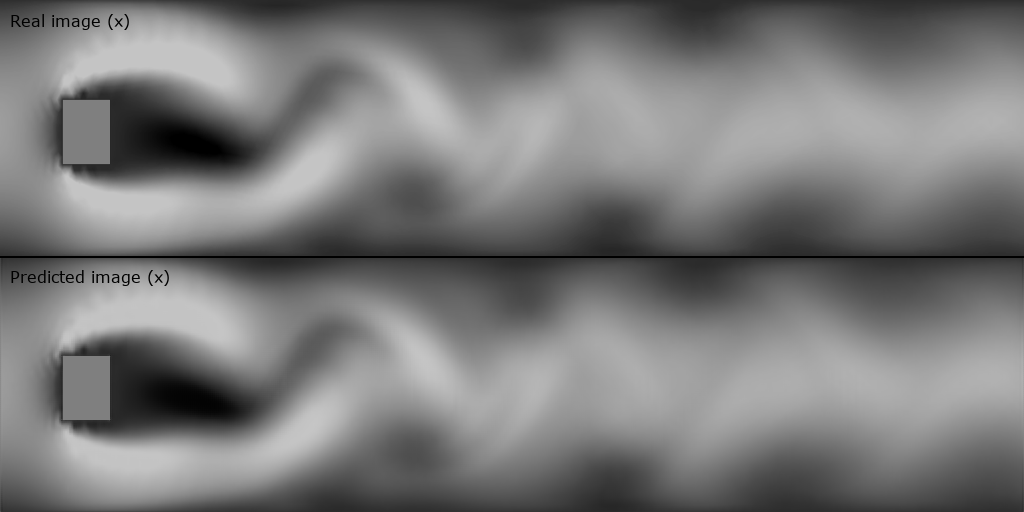
\includegraphics[width=1\linewidth]{imgs/pred}
  \end{subfigure}
  \begin{subfigure}{.5\textwidth}
    \centering
    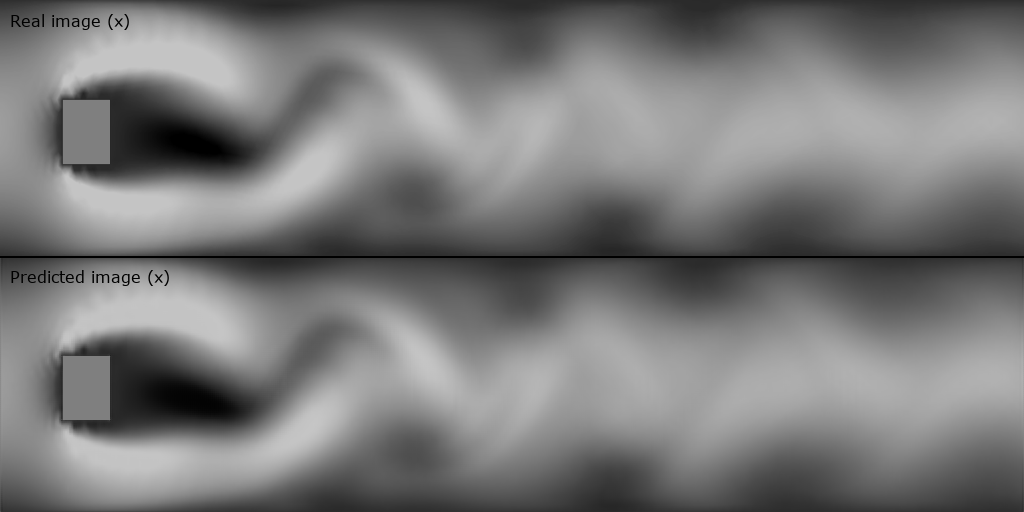
\includegraphics[width=1\linewidth]{imgs/pred.png}  
  \end{subfigure}
\end{figure}

The effects of the usage of the pressure field can be seen in the variance of the results. The pressure field has the potential to make the models better but in some runs it can also make them worse. We believe this is the case because the pressure fields increases the complexity of the data but it also carries information about the simulation that can be useful for the networks.

Based on our experiments, we can say that achieving good performance was the hardest for the constant model. We attribute that to the limited data with which it was trained --- only a single simulation. Contrary to the intuition, the more varied data is easier to predict, as it can be seen in the results for the inflow speed and viscosity-density models. We also believe, that a bigger test set can better estimate the performance of our models. This probably also contributes to the worse results for the constant models.

\noindent\textbf{Recursive Application Performance:}
With this evaluation case we want to see how our models handle recursive application. That is, the output of the network is used again as an input for the prediction of the next simulation frame.

For each recursive evaluation we generate 40 frames of the corresponding simulation. We did not in any was post-processed the output of the networks before feeding it as an input. We calculate the discussed metrics for each of the predicted frames while comparing them to the corresponding real one.

In our experiments, we performed several recursive evaluation for each simulation while starting at frames with different index. We wanted to see how a different starting point in the simulation can affect the frames predicted by the models.

The viscosity-density and inflow speed models are evaluated with several simulations with different parameters. As it is unpracticed to give the results of the evaluation of each simulation, here we present only several of them. The showed results, however, are representative of the general performance of our models. For this section, We also limit ourselves only to models that do use the pressure field of the simulations.

The constant model is evaluated with a single simulation --- the one it was trained with. [fig] presents the results of the recursive application. During the evaluation we noticed that the models can more accurately predict a simulation when the starting frame is further in the simulation. That is, its index relative to the first frame is higher. The plots for the constant model in [fig] illustrate this.

For the inflow speed model we present the results from three different simulations in [fig]. We can see the same trend that predicting frames with smaller index is harder. We, however, like to note that the networks appear to be handling the parameters properly and adjust the predicted frames accordingly. [fig] presents the results of the viscosity-density model.

We again do not explicitly give the correlation between the predicted and real frames. In all cases the correlation stayed very close to $1$ and varied in the range $[0.98, 0.99998]$. The CFD-metrics are summarized in [table]. 



\section{Conclusion}\label{conclusion}

\clearpage
\bibliographystyle{splncs04}
\bibliography{egbib}



\begin{subappendices}
\renewcommand{\thesection}{\Alph{section}}%

\section{Networks architectures and hyperparameters}
\emph{Here we give the exact details on the architectures of the used networks.}


\end{subappendices}


\end{document}

%%% Local Variables:
%%% mode: latex
%%% TeX-master: t
%%% End:

% LocalWords:  Convolutional timestep timesteps grayscale cGANs
